\chapter{Week14}
\section{Monday for MAT3040}\index{Monday_lecture}
\subsection{Multilinear Tensor Product}

\begin{definition}[Tensor Product among More spaces]
Let $V_1,\dots,V_p$ be vector spaces over $\mathbb{F}$.
Let $S=\{(v_1,\dots,v_p)\mid v_i\in V_i\}$
(We assume no relations among distinct elements in $S$), 
and define $\mathfrak{X}=\Span(S)$.
\begin{enumerate}
\item
Then define the tensor product space $V_1\otimes\cdots\otimes V_p=\mathfrak{X}/y$,
where $y$ is the vector subspace of $\mathfrak{X}$ spanned by vectors of the form 
\[
(v_1,\dots,v_i+v_i',\dots,v_p)
-
(v_1,\dots,v_i,\dots,v_p)
-
(v_1,\dots,v_i',\dots,v_p),
\]
and
\[
(v_1,\dots,\alpha v_i,\dots,v_p) - \alpha(v_1,\dots,v_i,\dots,v_p)
\]
where $i=1,2,\dots,p$.
\item
The tensor product for vectors is defined as
\[
v_1\otimes\cdots\otimes v_p:=\{(v_1,\dots,v_p)+y\}\in 
V_1\otimes\cdots\otimes V_p
\]
\end{enumerate}
\end{definition}
\begin{remark}
Similar as in tensor product among two space, 
\begin{enumerate}
\item
We have 
\[
v_1\otimes\cdots\otimes (\alpha v_i+\beta v_i')\otimes\cdots\otimes v_p
=
\alpha (v_1\otimes\cdots\otimes v_i\otimes\cdots\otimes v_p)
+
\beta (v_1\otimes\cdots\otimes v_i'\otimes\cdots\otimes v_p)
\]
\item
A general vector in $V_1\otimes\cdots\otimes V_p$ is 
\[
\sum_{i=1}^n
(W_1^{(i)}\otimes\cdots\otimes W_p^{(i)}),\quad
\text{where }
W_j^{(i)}\in V_j, j=1,\dots,p
\]
\item
Let $\mathcal{B}_i= \{v_i^{(1)},\dots,v_i^{(\dim(V_i))}\}$
be a basis of $V_i, i=1,\dots,p$,
then 
\[
\mathcal{B}
=
\{
V_1^{(\alpha_1)}
\otimes
\cdots
\otimes
V_p^{(\alpha_p)}
\mid 
1\le \alpha_i\le \dim(V_i)
\}
\]
is a basis of $V_1\otimes\cdots\otimes V_p$.
As a result,
\[
\dim(V_1\otimes\cdots\otimes V_p)
=
(\dim(V_1))\times\cdots\times
(\dim(V_p))
\]
\end{enumerate}

\end{remark}

\begin{theorem}[Universal Property of multi-linear tensor]
Let $\text{Obj}=\{\phi:V_1\times\cdots\times V_p\to W\mid\phi\text{ is a $p$-linear map}\}$, i.e.,
\begin{align*}
\phi(v_1,\dots,\alpha v_i+\beta v_i',\dots,v_o)
=
\alpha\phi(v_1,\dots,v_i,\dots,v_p)
+
\beta&\phi(v_1,\dots,v_i',\dots,v_p),\\
&\forall v_i,v_i'\in V_i,
i=1,\dots,p,
\forall\alpha,\beta\in\mathbb{F}.
\end{align*}
For instance, the multiplication of $p$ matrices is a $p$-linear map.

Then the mapping in the Obj, 
\[
\begin{array}{ll}
i:&V_1\times V_p\to V_1\otimes\cdots\otimes V_p\\
\text{with}&(v_1,\dots,v_p)\mapsto v_1\otimes \cdots\otimes v_p
\end{array}
\]
satisfies the universal property.
In other words, for any $\phi:V_1\times \cdots\times V_p\in\text{Obj}$, 
there exists the unqiue linear transformation 
\[
\bar{\phi}:V_1\otimes\cdots\otimes V_p\to W
\]
such that the diagram below commutes:
\begin{figure}[H]
\centering
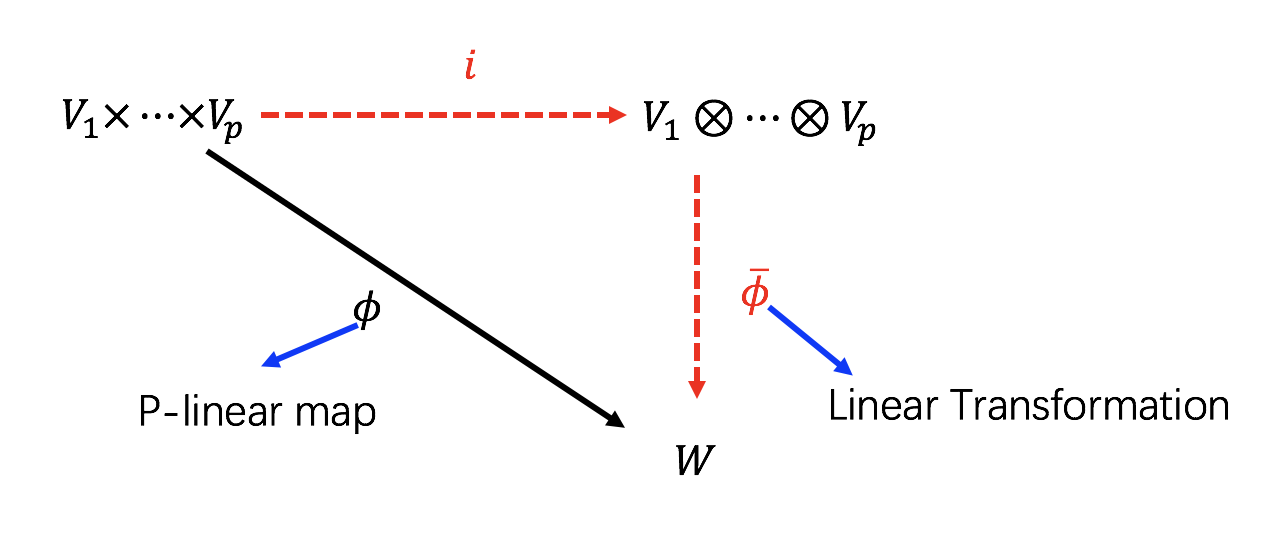
\includegraphics[width=0.6\textwidth]{week14/f_20}
\end{figure}
In other words, $\phi=\bar{\phi}\circ i$.
\end{theorem}

\begin{corollary}
Let $T_i:V_i\to V_i'$ be a linear transformation, $1\le i\le p$.
There is a unique linear transformation
\[
\begin{array}{ll}
(T_1\otimes\cdots\otimes T_p):&V_1\otimes\cdots\otimes V_p\to V_1'\otimes\cdots\otimes V_p'\\
\text{satisfying}&(T_1\otimes\cdots\otimes T_p)(v_1\otimes\cdots\otimes v_p)
=
T_1(v_1)\otimes\cdots\otimes T_p(v_p)
\end{array}
\]
\end{corollary}
\begin{proof}
Construct the mapping
\[
\begin{array}{ll}
\phi:&V_1\times\cdots\times V_p\to V_1'\otimes\cdots\otimes V_p'\\
\text{with}&(v_1,\dots,v_p)\mapsto T_1(v_1)\otimes\cdots\otimes T_p(v_p)
\end{array}
\]
which is indeed $p$-linear.

By the universal property, we induce the unique linear transformation
\[
\bar{\phi}:V_1\otimes\cdots\otimes V_p\to V_1'\otimes\cdots\otimes V_p'
\]
\end{proof}
\paragraph{Notation}
To make life easier, from now on, we only consider $V_1=\cdots=V_p=V$.
Then for any linear transformation $T:V\to W$, we have
\[
T^{\otimes p}:V\otimes\cdots\otimes V\to W\otimes\cdots\otimes W
\]
We use the short-hand notation $V^{\otimes p}$ to denote $\underbrace{V\otimes\cdots\otimes V}_{\text{$p$ terms in total}}$

\paragraph{Final Exam Ends Here}

\subsection{Exterior Power}

\begin{definition}
A $p$-linear map $\phi:V\times\cdots\times V\to W$ is called \emph{alternating} if
\[
\phi(v_1,\dots,v_i,\dots,v_j,\dots,v_p)=\bm0_{W},\quad
\text{provided that there exists some $v_i=v_j$ for $i\ne j$}.
\]
Also, we say $\phi$ is $p$-alternating
\end{definition}
\begin{example}
\begin{enumerate}
\item
The cross product mapping
\[
\begin{array}{ll}
\phi:&\mathbb{R}^3\times\mathbb{R}^3\to\mathbb{R}^3\\
\text{with}&(\bm v,\bm w)\mapsto\bm v\times\bm w
\end{array}
\]
is alternating:
\begin{itemize}
\item
$\phi$ is bilinear
\item
$\phi(\bm v,\bm v)=\bm v\times\bm v=\bm0$.
\end{itemize}
\item
The determinant mapping
\[
\begin{array}{ll}
\phi:&\underbrace{\mathbb{F}^n\times\cdots\times\mathbb{F}^n}_{\text{$n$ terms in total}}\to\mathbb{F}\\
\text{with}&(\bm v_1,\dots,\bm v_n)\mapsto\det([\bm v_1,\bm v_2,\cdots,\bm v_n])
\end{array}
\]
is alternating:
\begin{itemize}
\item
$\phi$ is $n$-linear by MAT2040 knowledge
\item
$\phi$ is alternating by MAT2040 knowledge
\end{itemize}
\end{enumerate}
\end{example}

\begin{theorem}[Universal Property for exterior power]
Let $\text{Obj}:=\{\phi:\underbrace{V\times\cdots V}_{\text{$p$ terms}}\to W\mid\phi\text{ is $p$-alternating map}\}$.
Then there exists $\{\Lambda:V\times\cdots\times V\to E\}\in\text{Obj}$ satisfying the following:
\begin{itemize}
\item
For all $\phi:V\times\cdots\times V\to W\in\text{Obj}$, there exists unique linear transformation $\bar{\phi}:E\to W$ satisfying 
\begin{figure}[H]
\centering
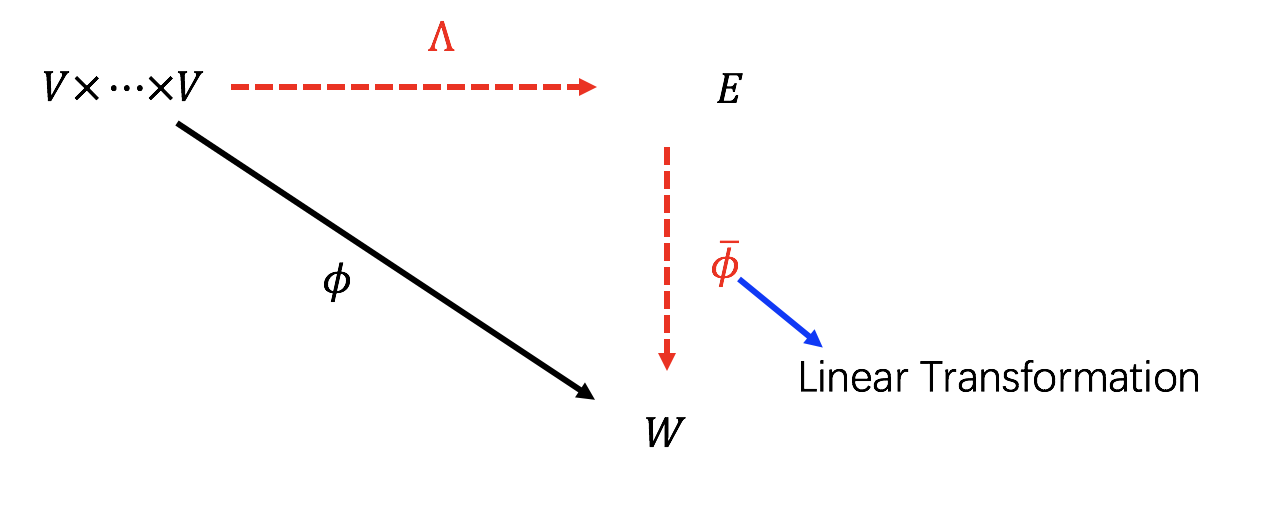
\includegraphics[width=0.6\textwidth]{week14/f_21}
\end{figure}
In other words, $\phi=\bar{\phi}\circ\Lambda$.
\end{itemize}
\end{theorem}












